\documentclass[conference]{IEEEtran}
\IEEEoverridecommandlockouts
% The preceding line is only needed to identify funding in the first footnote. If that is unneeded, please comment it out.
\usepackage{cite}
\usepackage{amsmath,amssymb,amsfonts}
\usepackage{algorithmic}
\usepackage{graphicx}
\usepackage{textcomp}
\usepackage{xcolor}
\usepackage{float}
\usepackage{subcaption}
\usepackage{graphicx}
\usepackage{tikz}
\usetikzlibrary{positioning}

\def\BibTeX{{\rm B\kern-.05em{\sc i\kern-.025em b}\kern-.08em
    T\kern-.1667em\lower.7ex\hbox{E}\kern-.125emX}}
\begin{document}

\title{Software Defined Radio Channel emulator for Satellite based GNSS communication systems initial report}

\author{\IEEEauthorblockN{George Burns}
\IEEEauthorblockA{\textit{dept. Electrical and Electronic Engineering} \\
\textit{University of Bristol}\\
Bristol, United Kingdom \\
george.burns.2001@bristol.ac.uk}
}

\maketitle

\begin{abstract}
This report will detail proposed methods to simulate radio frequency (RF) wave propagation of \textbf{$1G Hz$} too \textbf{$350G Hz$} satellite communication systems. It will detail the standards and mathematical models used to simulate some off the effects of on the propagation of RF waves through a Earth to space medium. There will also be detail on the modulation schemes used to test such simulation methods.
\end{abstract}

\section{Introduction}
In this section there will be a list of the effects that will be detailed in this report and simulated in the Channel Emulator. Satellite communications come under attenuation both complex and real. Most channel emulators for these effects are expensive and hard to implement however the aim of this projects is to construct software that simulates these effects.\\

Using \cite{seybold_introduction_2005} as a basic reference point a basic model can be constructed. As shown in Figure \ref{fig:System_model}. 
\begin{figure}[h]
\centering
	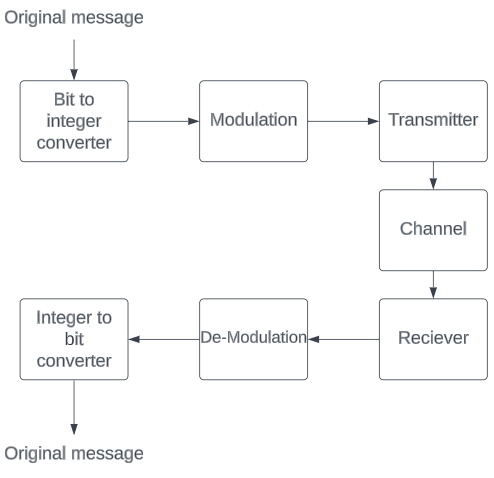
\includegraphics[width = 0.45\textwidth]{System_model.png}
	\caption{Full System Model}
	\label{fig:System_model}
\end{figure}

The Majority of the work will be focused on the Channel Emulator part of the system.\\

The Emulator will primarily focus on the following effects; Free space loss, Atmospheric Effects, Rain Fade, Noise Temperature, multipath fading and scintillation and the effects of orbit. All of these effects have a significant impact on the channel. They are both complex and real degradation. This means that for an electromagnetic wave represented as $Ae^{j w t+\theta}$, the channel will degrade the amplitude ($A$), the phase ($\theta$), and the frequency ($w = 2\pi f$), where $f$ is the frequency and $j= \sqrt{-1}$ is the imaginary number. These effects where chosen in accordance with \cite{kaplan_understanding_2017} which details these effects as being prominent in GNSS systems\\

These are also dependent on time as during the orbital period of the satellite both slant angle \cite{seybold_introduction_2005} and if the orbit is elliptical \cite{10.5555/2601574} the distance can also change, these effects will be detailed in section \ref{sec:7})
\label{sec:intro}


\section{Modulation}
A large variety of modulation schemes are used in satellite communications \cite{smith_modulation_2017}. For this project I will aim to employ multi-level frequency shift keying (MFSK) and multi-level amplitude shift keying (MASK) shown in both Figure \ref{fig:Moduluation_models}. This was a good way to progress onto more complicated modulation schemes like quadrature amplitude modulation (QAM).
\begin{figure}[h]
\centering
\begin{subfigure}{0.5\textwidth}
	\centering
	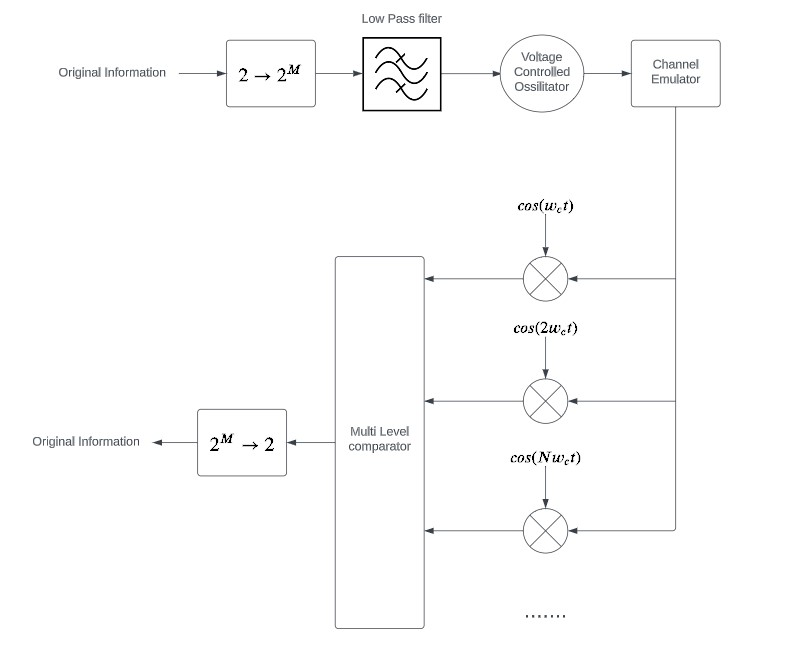
\includegraphics[width=\textwidth]{MFSK_model.png}
	\caption{MFSK Model}
	\label{fig:MFSK_model}
\end{subfigure}
\centering
\begin{subfigure}{0.5\textwidth}
	\centering
	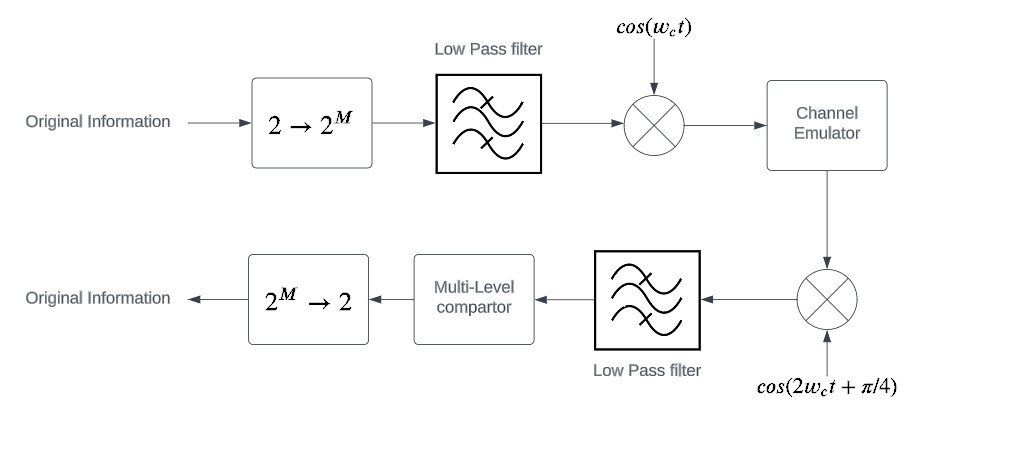
\includegraphics[width=\textwidth]{MASK_model.png}
	\caption{MASK Model}
	\label{fig:MASK_model}
\end{subfigure}
\caption{Modulation Schemes diagrams}
\label{fig:Moduluation_models}
\end{figure}
\label{sec:1}


\section{Free Space loss}
Equation \ref{eq:Free_space_equation} is used to model free space loss, $r_s$ is usually just distance on a terrestrial plane however slant path needs to be accounted for which can be calculated using Equation \ref{eq:Slant_path_equation}.\\
\begin{equation}
A_{fs} = \frac{A_r A_t}{\lambda^2 r_s^2}
\label{eq:Free_space_equation}
\end{equation}

Where $A_{fs}$ is free space loss, $A_r$ and $A_t$ are the area of transmitter and receiver antenna respectively $\lambda$ is wavelength and $r_s$ is slant path.\\


\begin{equation}
r_s = \frac{h sin(\psi)}{sin(\frac{\pi}{2}+\theta)}
\label{eq:Slant_path_equation}
\end{equation}

Where $h$ is the height above Earth, $r_e$ is Earth's radius $6378K m$, $\theta$ is the elevation angle and $\psi$ is the central angle determined by equation \ref{eq:Central_angle_equation}.\\

Thus as the satellite changes distance (slant path $r_s$) the free space attenuation changes. Other effects on this equation could be the frequency $f$ and thus the wavelength $\lambda$ of the radio frequency (RF) signal changing though the ionosphere mentioned in section X. 

\begin{equation}
\psi = cos^{-1}(\frac{r_e}{h}(sin(\frac{\pi}{2}+\theta))-\theta
\label{eq:Central_angle_equation}
\end{equation}

\label{sec:2}

\section{Atmospheric Attenuation}
Effects of the atmosphere along the slant path $r_s$ must be considered when modelling RF propagation through Earth's atmosphere, its effects can be mathematically modelled as having distinct layers. The full mathematical model is complex so the goal was to use the International Telecommunications Union's curve fitting process. Using \cite{ITU-R_P.676-5} to gain $\gamma_{o}$ the oxygen attenuation and $\gamma_w$ the water attenuation we can get an expression for atmospheric attenuation from \cite{ITU-R_P.618-7} to form equation \ref{eq:Atmospheric_attenuation_equation}.
\begin{equation}
A_a = \frac{h_o \gamma_o + h_w \gamma_w}{sin(\theta)}
\label{eq:Atmospheric_attenuation_equation}
\end{equation}
Where $A_a$ is the atmosphere attenuation in $dB$, $h_0$ is the oxygen height and $h_w$ is the water vapour height both obtained by using the curve fit equation found in \cite{ITU-R_P.618-7}.

\label{sec:3}

\section{Rain Attenuation}
Hydrometeors are small water particles in the atmosphere can cause RF attenuation and thus must be accounted for in the model ITU provides a suitable model where \cite{ITU-R_P.837-1} provides the $R_{0.001}$ rain statistic. Then in conjunction with \cite{ITU-R_P.618-7} we can develop the rain model necessary.\\

\label{sec:4}


\section{Scintillation}
Scintillation can both be accounted for using ITU recommendations in \cite{ITU-R_P.618-7} both for $\theta> 5°$ and $\theta < 5°$. These are all dependent on location and measurements from that area for parameters such as average humidity and temperature. For frequencies below $10G Hz$ Scintillation is more prevalent in the ionosphere and can be accounted for using \cite{ITU-R_P.531-14}.\\


\label{sec:5}

\section{Noise temperature}
The noise equation (equation \ref{:eq:Noise_equation}) states that noise is directly proportional to temperature. 
\begin{equation}
N = kT
\label{:eq:Noise_equation}
\end{equation}
Where $N$ is noise, $k$ is Boltzman's constant and $T[K]$ is temperature in Kelvin\\

Temperature can effected by a large array of systems and are detailed further in \cite{ITU-R_P.372-16}. The model I choose to implement is from \cite{ITU-R_P.618-7} and show in equation \ref{eq:Noise_temp_equation}
\begin{equation}
T_s = T_m(1-10^{-A/10})
\label{eq:Noise_temp_equation}
\end{equation}
Where $T_s[K]$ is the temperature seen at the antenna in kelvin, $A[dB]$ is path attenuation found in both \ref{sec:2} and \ref{sec:3} and $T_m [K]$ is the effective temperature in Kelvin.\\

Thus substituting $T_s$ in \ref{eq:Noise_temp_equation} with $T$ in \ref{:eq:Noise_equation} we can find a suitable value for noise in the system.

\label{sec:5}


\section{Doppler effect}
When an object is moving at high speeds it experiences the Doppler effect. To model this equation X can be used. 
\begin{equation}
f_{new} =(\frac{v_d+c}{v_s+c})f
\label{eq:Doppler_effect_equation}
\end{equation}
Where $f_{new}$ is the perceived frequency of the RF wave, $v_s$ is the speed of RF source, $v_d$ is the speed of receiver, $c$ is the speed of light in the medium and $f$ is the original frequency.\\

This equation is significant as the majority of the effects covered previously depend on the perceived frequency $f_{new}$. It also can cause issues for MFSK mentioned in section \ref{sec:1} as if there is a dramatic frequency shift in the RF signal bits can be perceived wrong when being de-modulated. This effect is extremely prevalent on systems where the speed of the source (satellite) is not constant during the orbital window as this can mean a frequency change during the pass and thus the de-coding system is time dependent thus this aspect of the project is extremely important.
\label{sec:6}

\section{Orbital considerations}
In previous sections particular attention has been paid to slant path $r_s$ this is especially important when considering satellite systems with elliptical orbits as the slant range is not constant for the orbital period. This no doubt changes a large amount of parameters outlines previously and the system becomes highly dynamic. 
\label{sec:7}
\bibliographystyle{IEEEtran}
\bibliography{My_Library}
\end{document}
